%! Author = rickr
%! Date = 11/17/2021
\section{Quantum Improvements}
	With the recent advancements in quantum computing, access to hardware has become readily available to the general public and quantum algorithms have been shown to perform exponentially better than some of their classical counterparts for select problems. 
	For example, Grover's algorithm can sort through and find an element within an unstructured set using $O(\sqrt{N})$ operations as oppose to the $O(N)$ performance of an exhaustive search. However, for many problems, it's is more beneficial to utilize techniques found in classical algorithms that take advantage of the structure of a problem. One such technique is Branch-and-bound. 
	By applying the Branch-and-Bound paradigm in a quantum setting, it is possible to achieve a near quadratic improvement beyond that of classical pruning techniques \cite{montanaro2020quantum}. 

	Though there are several different implementations of quantum computing systems, the most popular is the quantum circuit.
	The model is based on the concept of a qubit which is analogous to the bit in classical computing. 
	The qubit acts as the basic unit of quantum information and is physically realized as the spin state of a fermion (a particle with a half integer spin; typically 1/2). 
	Since the qubit is measured as the spin state of a particle, it's properties are governed by the wave function of that particle $|\Psi\rangle$. 
	For example, since the quantum spin number of a qubit is 1/2, it can exist in one of two states (spin up $|0\rangle$ or spin down $|1\rangle$) when measured. 
	However, before the measurement, the particle can be in a superposition of both states 
	\begin{equation}
		|\Psi\rangle = \alpha |0\rangle + \beta|1\rangle
		\label{eq:spinStates}
	\end{equation}
	where $\alpha$ and $\beta$ are probability amplitudes such that $|\alpha|^2+|\beta|^2 = 1$.
	It is only when the wave-function is measured that it actually collapse in a definite value of $|0 \rangle$ or $|1\rangle$.
	This means that unlike a classical bit that can discretely take on a value of $0$ \textit{or} $1$, the qubit can exist in a state of $0$ \textit{and} $1$ simultaneously. We can exploit this feature of quantum mechanics to increase the speed of classical algorithms by placing the qubit into a superposition of states and letting the system evolve in time before taking a measurement. 
	
	%! Author = rickr
%! Date = 11/27/2021
\subsection{Classical vs Quantum Walk}

Consider the case of a classical random walk. In this example we search for a marked node within a binary tree of size $n$ nodes. 
If we have no indication of where in the tree the target might be, then a sure proof way of finding it is to visit each node, one step at a time, with $50\%$ probability of taking a step to the left and $50\%$ probability of taking a step to the right. 
Naturally, for every step away from the origin, there is an equal probability of taking a step back toward the origin, and over time we will obtain a normal Gaussian distribution of steps as shown in Figure \ref{fig:quantumWalk}. 
The classical random walk distribution exhibits a variance of 
\begin{equation}
	\sigma^2 \propto n
\end{equation}
which is to say that there is a very low probability of hitting the target if it is far away from the origin.
Since  each step is based on a set of definite states, the randomness of the traversal is caused by a stochastic transition between states.
Now consider a random walk in a quantum setting. 
In this case, the randomness comes from the quantum superposition imposed by Equation \ref{eq:spinStates}, a reversible unitary evolution (typically in the form of a Hadamard coin), and a collapse of the wave-function when a measurement is actually taken. 
Another difference between the quantum and classical random walk is the time at which a measurement is taken. 
In the classical version, it makes no difference to take measurements at each iteration, however in the quantum version, if a measurement of the wave-function is taken at each iteration, then the distribution converges to the classical Gaussian form. 
If the wave-function is left to interfere with itself before a measurement is taken, then the probability distribution is much more intricate, as can be seen in Figure \ref{fig:quantumWalk}.
It can be shown the after $n$ steps, the quantum walk obtains a variance of 
\begin{equation}
	\sigma^2 \propto n^2 \quad\cite{kempe2003quantum}
\end{equation}
Therefore, the quantum walk propagates quadratically faster than the classical walk, and this speed increase can be applied to the branch-and-bound framework. 
From Figure \ref{fig:quantumWalk}, if the wave-function is placed in a superposition, then the distribution exhibits destructive interference about the origin.
However, if the wave-function begins in a pure spin-up or spin-down configuration, then it is possible to create a bias toward any particular direction as shown in Figure \ref{fig:biasWalk} of the appendix.
\begin{figure}[H]
	\begin{center}
		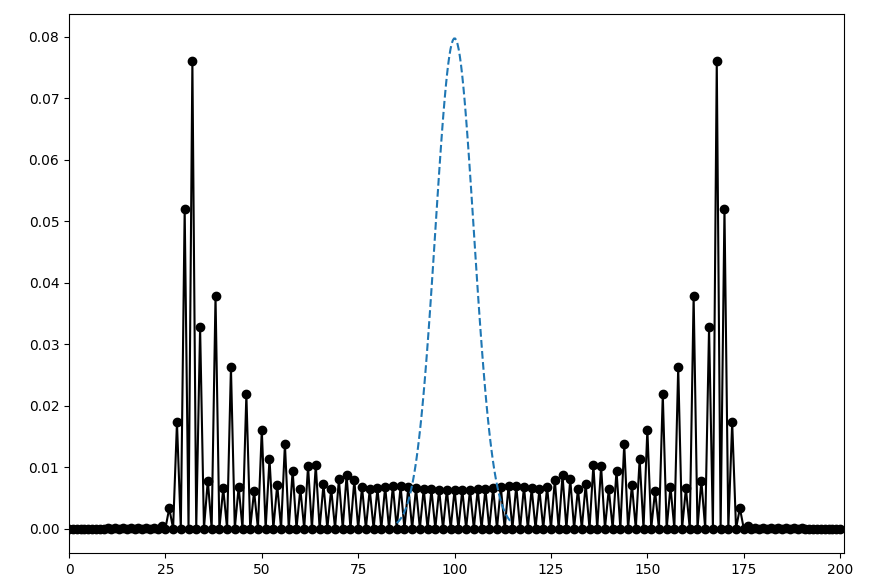
\includegraphics[width=12cm]{images/afunc2}
	\end{center}
	\caption{\doublespacing Difference between quantum and classical random walk. The blue dotted line represents the Gaussian distribution created by the classical walk and has a variance $\sigma^2 \propto n$. The black distribution is the result of the quantum random walk where the initial wave-function placed into a superposition $|\Psi\rangle = \alpha|0\rangle + \beta|1\rangle$ and acted on my a balanced Hadamard coin. The quantum distribution exhibits a variance of $\sigma^2 \propto n$ with de-constructive interference about the origin and constructive interference at the edges of propagation.}
	\label{fig:quantumWalk}
\end{figure}
\noindent
To summarize the results, consider three individual cases of solving combinatorial problems with Hamiltonians similar to that of Equation \ref{eq:isingHamiltonian}.
One case is solved using classical branch-and-bound techniques, one is solved using quantum walks, and one is solved using branch-and-bound in a quantum setting. 
If the classical branch-and-bound techniques are applied to solve for the largest known ground states of the Beransconi model, the runtime is roughly $O(2^{0.79n})$ \cite{packebusch2016low}. 
If we apply a quantum walk to classical algorithms that solve the Sherrington-Kirkpatrick model (an Ising model with long range anti-ferrmagnetic couplings) then it has been shown we can increase runtime to approximately $O(2^{0.41n})$ \cite{callison2019finding}. 
Finally, by applying quantum branch-and-bound algorithms to the same model, it has been shown that the runtime can be increased further to $O(2^{0.226n})$ \cite{montanaro2020quantum}.
